\begin{frame}{}

\huge{Use cases}

\end{frame}

%------------------------------------------------------------
\begin{frame}{Reproducibility - how far and for what?}
\begin{center}
    
\includegraphics[height=3cm]{shared/FAIR_equilibre.png}\\
    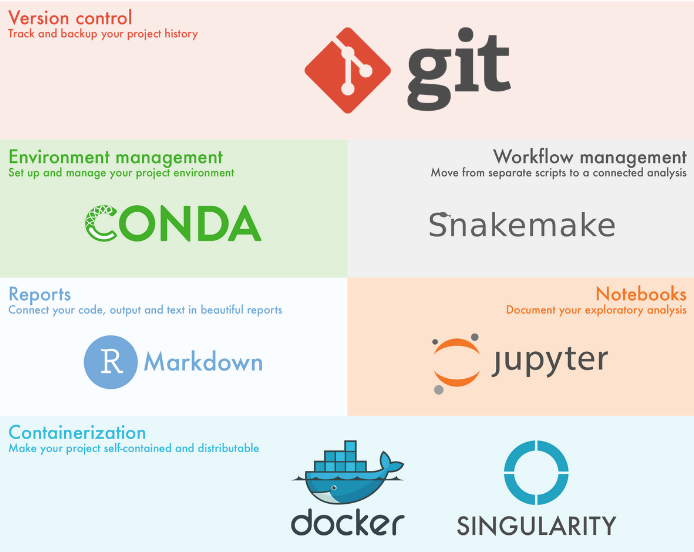
\includegraphics[width=3cm]{10_usecases/images/FAIR_NBIS_tools.png}
    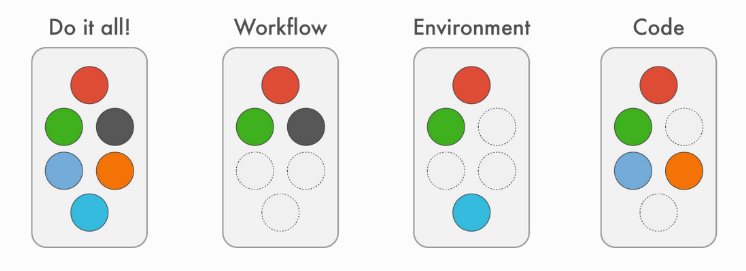
\includegraphics[width=8.5cm]{10_usecases/images/FAIR_NBIS_pastilles.png}
    \href{https://nbis-reproducible-research.readthedocs.io/en/latest/}{\textcolor{blue}{nbis-reproducible-research.readthedocs.io/en/latest}}
\end{center}
\end{frame}
%------------------------------------------------------------
\begin{frame}{Reproducibility tools}
Coloured dots: symbolise tools \\
Variable intensities: according to expertise\\
not needed, basic use, advanced use (expert)
\begin{center}
\begin{tabular}{|c|c|c|}
   \hline
   \includegraphics[height=0.7cm]{shared/logo-git.png} & 
\includegraphics[height=0.7cm]{10_usecases/images/FAIR_dots_git.png} & clone branch \\
   \includegraphics[height=0.6cm]{shared/logo-github.png} & 
\includegraphics[height=0.7cm]{10_usecases/images/FAIR_dots_github.png} & collaborate pages (actions)\\
   \includegraphics[height=0.4cm]{shared/logo-conda.png} & 
\includegraphics[height=0.7cm]{10_usecases/images/FAIR_dots_conda.png} & install yml (recipe)\\
   \includegraphics[height=0.7cm]{shared/logo-docker-paysage.png}, \includegraphics[height=0.6cm]{shared/logo-singularity.png} & 
\includegraphics[height=0.7cm]{10_usecases/images/FAIR_dots_docker.png} & run dockerfile\\
   \includegraphics[height=0.7cm]{shared/logo-snakemake.png} & 
\includegraphics[height=0.7cm]{10_usecases/images/FAIR_dots_smk.png} & run snakemakefile\\
   \includegraphics[height=0.6cm]{shared/logo-jupyter.png}, \includegraphics[height=0.6cm]{shared/logo-Rmarkdown.png} & 
\includegraphics[height=0.7cm]{10_usecases/images/FAIR_dots_jupyter.png} & run notebookfile \\
   \includegraphics[height=0.7cm]{shared/logo-zenodo.png} & 
\includegraphics[height=0.7cm]{10_usecases/images/FAIR_dots_zenodo.png} & download submit\\
   \hline
\end{tabular}
\end{center}
\end{frame}
%------------------------------------------------------------
\begin{frame}{Use cases}
\begin{block}{What we learned during the courses}
\begin{columns}
\begin{column}{0.3\textwidth}
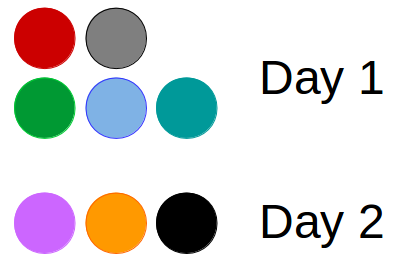
\includegraphics[height=2cm]{10_usecases/images/FAIR_dots_formation.png}
\end{column}
\begin{column}{0.65\textwidth}
Day 1: Git (advanced), Github (basic), conda (advanced), zenodo (basic), docker (advanced)\\
Day 2: snakemake (advanced), jupyter (advanced), github (advanced)
\end{column}
\end{columns}
\end{block}
\begin{exampleblock}{Brainstorming}
Choose coloured dots for tools to represent:
\begin{itemize}
    \item Daily use
    \item Share an analysis with colleagues or your supervisor (they may want to perform)
    \item A part of the material and method for a publication 
\end{itemize}
\end{exampleblock}
\end{frame}